\documentclass[letter,onecolumn,12pt]{aiaa-tc}


\usepackage{color}
\usepackage[T1]{fontenc}
\usepackage[sc]{mathpazo}
\usepackage{caption}
\usepackage{subcaption}
\usepackage{blkarray}
\usepackage{paralist}
\usepackage{dsfont}
\usepackage{bm}
\usepackage{soul}
\usepackage{url}
\usepackage[cmex10]{amsmath}
%\usepackage{hyperref}
%\usepackage{breakurl} % this cuts urls in a nice way so that they don't go out of the margins

%\usepackage[intlimits,cmex10]{amsmath}
\interdisplaylinepenalty=2500
\usepackage{amssymb}
\usepackage{floatflt}
\usepackage{epsfig,psfrag,graphicx,wrapfig}
%\usepackage[caption=false,font=footnotesize]{subfig}% subcaptions for subfigures
\usepackage[colorlinks]{hyperref}%  hyperlinks [must be loaded after dropping]
\usepackage{cite}
%\usepackage{refcheck}



% -----   NEW COMMANDS & ENVIRONMENTS   ----------------------------------------
%
\newcommand{\Lone}{\mathcal{L}_1}
\newcommand{\Linf}{\mathcal{L}_{\infty}}
\newcommand{\Lonenorm}[1]{\ensuremath{\left\Vert{#1}\right\Vert_{\mathcal{L}_1}}}
\newcommand{\Linfnorm}[1]{\ensuremath{\left\Vert{#1}\right\Vert_{\mathcal{L}_{\infty}}}}
\newcommand{\Linfnormt}[2]{\ensuremath{\left\Vert{#1}_{#2}\right\Vert_{\mathcal{L}_{\infty}}}}
\newcommand{\lonenorm}[1]{\ensuremath{\Vert{#1}\Vert_{\mathcal{L}_1}}}
\newcommand{\linfnorm}[1]{\ensuremath{\Vert{#1}\Vert_{\mathcal{L}_{\infty}}}}
\newcommand{\linfnormt}[2]{\ensuremath{\Vert{#1}_{#2}\Vert_{\mathcal{L}_{\infty}}}}
\newcommand{\Infnorm}[1]{\ensuremath{\left\Vert{#1}\right\Vert_{\infty}}}
%\newcommand{\Twonorm}[1]{\ensuremath{\left\Vert{#1}\right\Vert_{2}}}
\newcommand{\Twonorm}[1]{\ensuremath{\left\Vert{#1}\right\Vert}}
\newcommand{\Onenorm}[1]{\ensuremath{\left\Vert{#1}\right\Vert_{1}}}
\newcommand{\Abs}[1]{\ensuremath{\left|{#1}\right|}}
\newcommand{\infnorm}[1]{\ensuremath{\Vert{#1}\Vert_{\infty}}}
%\newcommand{\twonorm}[1]{\ensuremath{\Vert{#1}\Vert_{2}}}
\newcommand{\twonorm}[1]{\ensuremath{\Vert{#1}\Vert}}
\newcommand{\onenorm}[1]{\ensuremath{\Vert{#1}\Vert_{1}}}
\newcommand{\abs}[1]{\ensuremath{|{#1}|}}

\newcommand{\trace}[1]{\ensuremath{{\rm tr}\left[{#1}\right]}}
\newcommand{\Proj}[3]{\ensuremath{{\rm Proj}_{#1}({#2},{#3})}}
\newcommand{\Exp}[1]{\ensuremath{{\rm e}^{{#1}}}}
\newcommand{\Inv}[1]{\ensuremath{\left({#1}\right)^{-1}}}
\newcommand{\inv}[1]{\ensuremath{({#1})^{-1}}}

\newcommand{\drv}[2]{\frac{{\rm d}{#1}}{{\rm d}{#2}}}
\newcommand{\sat}[1]{\ensuremath{\operatorname{sat}\left({#1}\right)}}

\newcommand{\IR}{\mathds{R}}
\newcommand{\IZ}{\mathds{Z}}

\newcommand{\II}{\mathds{I}}
\newcommand{\IIn}[1]{\mathds{I}_{\bm{#1}}}

\newcommand{\matt}[1]{\begin{bmatrix}#1\end{bmatrix}}
\newcommand{\smatt}[1]{\left[\begin{smallmatrix}#1\end{smallmatrix}\right]}
\newcommand{\1}{1_n}
\newcommand{\col}{\operatorname{col}}
\newcommand{\card}{\operatorname{card}}

\newcommand{\Acal}{\mathcal{A}}
\newcommand{\Bcal}{\mathcal{B}}
\newcommand{\Ccal}{\mathcal{C}}
\newcommand{\Dcal}{\mathcal{D}}
\newcommand{\Ecal}{\mathcal{E}}
\newcommand{\Fcal}{\mathcal{F}}
\newcommand{\Gcal}{\mathcal{G}}
\newcommand{\Hcal}{\mathcal{H}}
\newcommand{\Ical}{\mathcal{I}}
\newcommand{\Jcal}{\mathcal{J}}
\newcommand{\Kcal}{\mathcal{K}}
\newcommand{\Lcal}{\mathcal{L}}
\newcommand{\Mcal}{\mathcal{M}}
\newcommand{\Ncal}{\mathcal{N}}
\newcommand{\Ocal}{\mathcal{O}}
\newcommand{\Pcal}{\mathcal{P}}
\newcommand{\Qcal}{\mathcal{Q}}
\newcommand{\Rcal}{\mathcal{R}}
\newcommand{\Scal}{\mathcal{S}}
\newcommand{\Tcal}{\mathcal{T}}
\newcommand{\Ucal}{\mathcal{U}}
\newcommand{\Vcal}{\mathcal{V}}
\newcommand{\Wcal}{\mathcal{W}}
\newcommand{\Xcal}{\mathcal{X}}
\newcommand{\Ycal}{\mathcal{Y}}
\newcommand{\Zcal}{\mathcal{Z}}
% ------------------------------------------------------------------------------


\graphicspath{{./figures/}}

\renewcommand{\baselinestretch}{1}



% ==============================================================================
% =====   PROPOSAL BEGINS HERE   ===============================================
% ==============================================================================
\begin{document}


\pagestyle{empty}
%==============================================================================
\section*{Executive Summary}  %<= 4,000 characters
%==============================================================================

%------------------------------------------------------------------------------
\textbf{\emph{Objective}:} The proposed research will develop an analytical framework for assessing the impact
of mis-communication or low-connectivity conditions on the automated separation assurance of multiple cooperative
airplanes sharing the same airspace. The Intergraded Separation Assurance In Low-Connectivity (iSEALC) framework
is a solution of future high-density self-separating airflow envisioned by NextGen. iSEALC framework is based on
the notion of  multiple cooperative aircraft flying along their parameterized routes and sharing their state
and intent information. The framework takes into account the switching topology and possibly degraded connectivity
of the existing communication networks defined for NextGen and performance characteristics of heterogeneous aircraft.
%The ultimate goal of the iSEALC framework is to provide a rapidly accessible and verifiable tool for assessing the separation guarantees of a given number of airplanes in a given ATC sector with degraded communication capabilities.
%The tool is  envisioned first to be integrated into existing mode of air traffic management as an advisory aid. At the second phase the distributed coordination algorithm can be implemented onboard thus enabling automation of the path following and coordination.
The technical challenges that will be addressed are the four subtopics of AFSC-1.5:
\vspace{-2mm}
\begin{itemize}
\setlength{\itemsep}{-4pt}
    \item formalize the failure space of individual and integrated communication technologies,
    \item design the loss of separation metrics and a unified distributed mitigation mechanism,
    \item analyze the impact of  communication constraints onto the separation assurance, and
    \item develop a mechanism by which degraded communication and associated detection and mitigation strategies will guarantee separation assurance.
\end{itemize}
\vspace{-2mm}
%--------------------------  FIGURE  ------------------------------------------
\begin{wrapfigure}{r}{0.55\textwidth}
\centering
\vspace{-0mm}
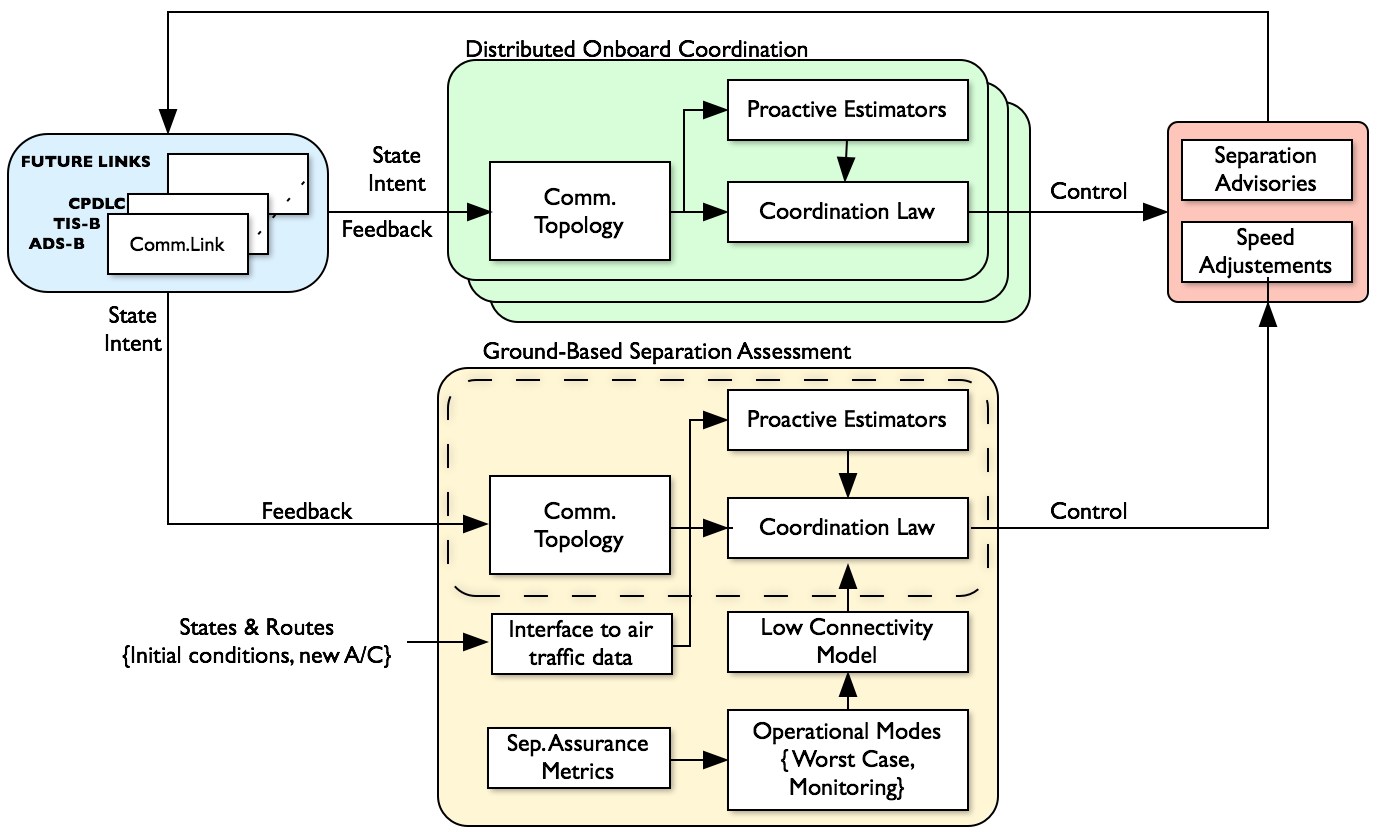
\includegraphics[angle=0,width=0.55\textwidth,]{iSEALC.eps}
\caption*{\footnotesize iSEALC: \textbf{I}ntegrated \textbf{Se}paration \textbf{A}ssurance in \textbf{L}ow \textbf{C}onnectivity conditions.}
\label{fig:ISEALC}
\end{wrapfigure}
%------------------------------------------------------------------------------
\vspace{-1mm}

Research will build upon past expertise with the Coordinated Path Following (CPF) of Multiple UAVs project and
the use of novel adaptive control strategies to ensure a predictable response of a system of multiple aircraft
sharing the same airspace in the presence of adverse communication conditions.
%The adverse communication conditions were defined by the degradation of the quality of communicated states which uniquely identify relative position and intent of the airplanes along their routes.
%This quality IS defined by the completeness of the state vector that specifies the state of the aircraft (position, speed course, trajectory angle, intent), the update rate of communicating the states across the network, and the network topology that might have disconnected segments. Special emphasis will be placed on the cumulative (over time) degradation of the communication topology and advanced algorithms of estimating of partially-communicated states across the time-varying network.
The solution is based on transforming the key theoretical results of the CPF framework that is based on the 4D notion of trajectory representation; the trajectory consists of the 3D analytical path and the 1D velocity profile associated with the path. Multiple aircraft can safely follow the same paths that intersect in space but are still separated in time.

%The CPF concept naturally fits the NextGen 4D notion of the airspace utilization; the CPF fundamental results are a perfect match for the key objectives of the nation-wide program.

\medskip

%------------------------------------------------------------------------------
\textbf{\emph{Expected Outcomes and Benefits}:} The key outcome is the iSEALC system (depicted in the figure). For a given ATC sector the system will ``ingest'' the current ATC status (class and geometry of the segment, number and type of airplanes along with the assigned routes,  the communication links of aircraft and ground support infrastructure) and produce a detailed report addressing possible separation assurance violations and remedies (controls).

%The report will address the following:
%\begin{itemize}
 %   \setlength{\itemsep}{-4pt}
%	\item possible violations of separation assurance with identification of specific routes and airplanes involved,
%   	\item proposed strategies to eliminate the separation faults expressed as adjustments of the speed control laws for each of the airplanes potentially involved in a collision,
%    	\item ability to submit this strategies onboard of airplanes for timely execution,
%    	\item ability to execute the iSEALC system algorithms either on the ground as an %assessment tool or to implement it onboard as a part of a pilot advisory system in a %distributed fashion to facilitate any desired level of automation.
%\end {itemize}

%The following algorithms will be developed: $(i)$~the algorithms for detection of possible separation violations that identify the routes and the aircrafts involved; $(ii)$~the prioritization algorithms that produce a time-ordered sequence of possible violations; $(iii)$ - the recommended speed control laws capable to eliminate the violations; $(iv)$~the estimation algorithms that predict the position of neighboring airplanes which do not communicate their states. The main benefit will be a \emph{safer} automatic separation assurance system as envisioned under the NextGen concept in the 2025 time frame.

\medskip

%------------------------------------------------------------------------------
\textbf{\emph{Relevance to NASA Strategic Plan}:} The proposed research develops novel distributed control
architecture that facilitates automation in airspace management while preserving robust separation assurance
properties through scalability and cooperative computation. The proposed framework  assures safe operation under the communication technologies  and the air traffic mode of operation defined for NextGen.
%Besides compliance with current state of the art in NAS, the iSEALC framework perfectly matches the NextGen concept through applying its 4D-based trajectory representation, relying on distributed communication and computational capabilities that provide unprecedented scalable benefits and efficiency for the increased capacity of future NAS.
The proposed framework addresses the fundamental objectives of Subtopic~\mbox{AFCS-1.5} that is a part of the System-Wide Safety Assurance Technologies project  announced by the NASA Aeronautics Research Mission Directorate in support of NASA Strategic Goal~4 and Outcomes~4.1 and 4.2.

% ===== end Executive Summary   ===============================================



\clearpage
\thispagestyle{empty}
% =============================================================================
\tableofcontents
% =============================================================================



\clearpage
\pagestyle{plain}
\pagenumbering{arabic}
% =============================================================================
% === TECHNICAL SECTION (max 20 pages)   ======================================

% =============================================================================
\section{Objectives of the Proposed Research}
% =============================================================================

The main objective of this research is to develop assessment and mitigation tool and methods of automatic separation assurance which will provide provable evidence of a desired level of safety of multiple cooperative airborne aircraft in the presence of degraded or intermittently lost communication. Degraded or even lost communication with air traffic controllers is one of the major reasons of fatal aircraft accidents~\cite{Kochenderfer_2012}. The proposed  Intergraded Separation Assurance In Low-Connectivity (iSEALC) framework takes into account the switching topology and possibly degrading connectivity of the existing communication networks and the flight characteristics of heterogeneous airplanes. The key enabling blocks of the iSEALC framework are the distributed coordination law and the set of proactive state estimators that enable self-separating cooperative flow of multiple aircraft in the presence of severely degraded communication.

The ultimate goal of the iSEALC framework is to provide a rapidly accessible and verifiable tool for assessing the separation guarantees of a given number of airplanes in a given ATC sector with degraded communication capabilities.  The tool is  envisioned initially to be integrated into existing mode of airspace management as an advisory aid. At the second phase the distributed coordination algorithms can be implemented onboard thus enabling automation of the route following and coordination. The technical challenges that will be addressed with iSEALC are the four subtopics of AFSC-1.5:
\vspace{-2mm}
\begin{itemize}
\setlength{\itemsep}{-4pt}
    \item formalize the failure space of individual and integrated communication technologies,
    \item design the loss of separation metrics and a unified distributed mitigation mechanism,
    \item analyze the impact of  communication constraints onto the separation assurance, and
    \item develop a mechanism by which degraded communication and associated detection and mitigation strategies will guarantee separation assurance.
\end{itemize}
\vspace{-2mm}

The adverse communication conditions are defined by the degradation of the quality of communicated states which uniquely identify relative position and intent of the airplanes along their routes. This quality is defined by the completeness of the delivered state vector that specifies the state of the aircraft (position, speed course, trajectory angle, intent), the update rate of communicating the states across the network, and the network topology that might have disconnected segments. Special emphasis will be placed on the cumulative (over time) loss of the communication and its impact on the degradation of separation assurance bounds. Addressing adverse effects of loss of communication, the research will also develop novel algorithms of estimating of partially-communicated states across the time-varying network.

The following algorithms will be developed: $(i)$~the algorithms for detection of loss of separation that identify the corresponding routes and the aircrafts involved; $(ii)$~the prioritization algorithms that produce a time-ordered sequence of possible violations; $(iii)$ - the recommended speed control laws capable to eliminate the violations; $(iv)$~the estimation algorithms that predict the position of neighboring airplanes which do not or partially communicate their states. The main benefit will be a \emph{safer} automatic separation assurance system as envisioned under the NextGen concept in the 2025 time frame.

We believe that integrating iSEALC architecture will be constructive in fundamentally improving situation awareness of all participants of the airflow process and improve overall safety of NAS operation.

% ===== end Objectives   ======================================================

% =============================================================================
\section{Technical Approach and Methodology}
% =============================================================================

% -----------------------------------------------------------------------------
\subsection{Motivation and Background}
% -----------------------------------------------------------------------------
In 2006 it was estimated~\cite{FAA_ATO_2006} that there were about 7,000 aircraft occupying national airspace (NAS) at any given time. This number implies that there are almost 50,000 aircraft transiting the NAS everyday. The airspace is busy being constantly under stress and diverse set of adverse conditions coming from both the human and technological factors, as well as from the environment. Although the rate of air traffic control (ATC) errors of various categories remains low,  when taken cumulatively over a longer period of time, the dynamics of the ATC error rate in 2006 indicate a $68\%$  increase when compared to those reported in 1998~\cite{USAToday_2006}. According to FAA statistics, the number of reported operational errors increased by more than 50 percent between fiscal years 2009 and 2010. Thus, considering a constantly increasing air traffic density, this positive trend in ATC and operational error rates might result in a serious increase in the number of accidents in near future.

One of the parameters defining the safety of flight is the separation distance between aircraft. To help maintaining safe separation distances between aircraft, while under the control of ATC personnel, the Federal Aviation Administration (FAA) established minimum separation standards based on the aircraft phase of flight and size. The ATC airspace surveillance infrastructure and controllers are responsible for providing instructions and advisories to pilots.

Loss of standard separation (LOS) is an event when aircraft do not maintain the minimum distance apart. Despite significant efforts of a number of government authorities including the FAA and the National Transportation Safety Board (NTSB) the violation of LOS constraints still remains a significant safety concern~\cite{OIG_AR2013}. If unobserved or not timely and properly addressed the LOS encounter may result in near midair collisions and midair collisions (MAC) between aircraft in flight. Note, that most MAC incidents are direct results of LOS occurrence, while not every LOS event leads to a collision. On the same note, a MAC is an event observed and reported by a pilot that is based solely on a pilot's perspective, not on hard data. A loss of separation is based on hard data obtained by various instrumentation including radar data and their factual measurements that are thoroughly tracked.

First, it is worth illustrating the widespread of LOS events and the general nature of their causes. In January 2011, an ATC \emph{operational error} led to a LOS that resulted in a near mid-air collision  between a commercial airliner and two military aircraft near New York City. According to the NTSB\cite{OIG_AR2013}, who investigated the incident, at their closest proximity, the aircraft came within a mile of each other while 3 miles were required. There was no single point of failure identified as a result of the investigation but a \emph{sequence} of steps that led to the LOS event. Since a number of instruments onboard and on the ground provided the telemetry of close proximity flight, the responsibility for the incident was assigned to the ATC personnel and the pilots.

On February 6, 2013  a number of  passenger planes were involved in a serious LOS incident in Finland~\cite{Vantaa_IR2013}.  Three civil aircraft were on approach to runway at Helsinki-Vantaa Airport; Norwegian Boeing-737, was on final approach, followed by a Flybe Nordic ATR, and a British Airways Airbus A320. A \emph{sequence of uncoordinated events} between aircrafts and the ATC controller cased two sequential breaches of separation minima between each aircraft in pairs. Although there was no risk of collision according to the Safety Investigation Authority of Finland~\cite{Vantaa_IR2013}, the LOS event was classified as a 'serious incident'.

On July 29th, 2011, a loss of separation occurred between two Boeing-737 aircrafts in the holding pattern at 93 miles south-west of Brisbane, Queensland\cite{Brisbane_ATSR2011}. The aircraft were inbound to Brisbane airport on the same air route, with a requirement to hold at Brisbane approach for sequencing. The air traffic controller did not identify that the sequence in which the two aircraft entered the holding pattern had changed, and twice assigned one of the aircraft descent through the flight level of another. The flight crew of lower flying aircraft identified the conflict and queried the controller, who then took action to recover the compromised separation situation. During the LOS event the separation reduced to 3.9 miles and 400 ft, while the required separation standard was 5 miles and 1000 ft. The Australian transport safety bureau identified that the controller was \emph{insufficiently trained}, and had not consolidated effective control techniques for the sector, particularly for high-workload situations.

These examples present very limited information taken primarily from the high-end instrumented aircraft and sufficient level of ATC support. However they do illustrate that the general practices and regulations tend to assign human error as the primary cause for the LOS incident. While the required human training and staffing side is taken care by a number of FAA procedural changes and regulations\cite{OIG_AR2013} the lack of technology support is also evident. The number and variety of disparate sources of information characterizing excessively complex airspace require significant automation to be developed in support of airspace management. The algorithms of predicting potential LOS event for much longer time, possibly up to the remaining flight duration, as a desired metric still need to be developed. Automatic assignment of en route and terminal approach sequencing of aircraft need to be automated and made dependent on the performance and equipage of the aircraft. The strategies accounting for the degraded communication among the ATC personnel on the ground and the airborne aircraft need to be developed.

At the same time, it also clear that there is no seldom single cause for an aircraft separation violation as it is usually a result of  a sequence of events triggered at a relatively late stage of close proximity encounter - last 3 to 10 minutes. This late stage of LOS detection is the result of lack of a unified system that would be able to ''ingest`` disparate data about all airborne vehicles and track the progression of all aircraft in the air while providing coordination command to the neighboring aircraft and shared access to this data to the entire fleet.

It is important to observe that although the current mode of airspace management assumes detailed knowledge of flight plan of every commercial aircraft that includes the detailed route and assigned speed profile, yet the LOS and MAC events happen. The probability of these events is unevenly shared between the en route and terminal airspace segments with the latter one contributing the vast majority of the occurrences; various sources including government authorities, industry and private sector provide inconsistent and therefore significantly ranging data, however the dominance of terminal airspace is obvious.

Furthermore, it is evident that ATC controllers have access to enormous amount of information obtained by disparate sources. Although supported by a number of technologies it is still their responsibility to fuse heterogeneous sources of information, interpret and keep updating the situational awareness so that their advisories to the crew are timely and unambiguous. On the other hand, the pilots have significant degree of freedom of interpretation of the advisories and the onboard instrumentation readings. Thus, being under stress of close proximity flight, they are often confused with frequent advisories~\cite{Kochenderfer_2012} given by the onboard systems ( various Collision Avoidance Systems (CAS) like TACAS, ACAS, ACASx) on one hand and the instructions received from the ATC controllers on the other. When overloaded, the pilot is likely to make a mistake leading to fatal consequences. Therefore, although human errors are the biggest contributors to the LOS accidents, the current operational load of ATC controllers and pilots is approaching its limit. There is obvious need not only to automate the heterogeneous information fusion but also to develop tools and methods that would detect the possibility of LOS way ahead of its occurrence.

%As a result this separation of responsibilities, the most LOS events are classified as an  \emph{operational error} ,when the controller's actions caused the loss, while if the pilot's actions caused the LOS it is classified as a pilot \emph{deviation} and are not typically associated with errors caused by the situational awareness (instruments and algorithms) and data communication infrastructure.

Prevention of separation violation accidents becomes even more crucial in future airspace operations under the NextGen Air Transportation  System~\cite{NextGen_ConOps}. The NextGen concept envisions highly-integrated airspace operations in the 2025 time frame, necessary in order to cope with the rapid growth of air travel and operational diversity. The NextGen concept of operations includes high-density, all-weather, and self-separation operational concepts, and is also expected to allow mixed-capability aircraft to operate within the same airspace, including piloted aircraft and unmanned aircraft systems. Solution to this growing demand for high density self-separated airflow is in distributed automation that allows for desired scalability of algorithms and guarantees high robustness of the entire airspace management system to a failure of its single element.

%%Formulate the problem that was addressed by the old technologies. Highlight what is wrong with that setup.

%ClosestProximity - The smallest distance ( point-to-point straight line in space) between two aircraft during an airborne loss of standard separation occurrence, regardless of geometry or percent of separation remaining.

%Measure of Compliance (MOC) - During a loss of standard separation occurrence involving radar separation minima for which recorded radar data is available, the greatest percentage of remaining separation (vertical or lateral) at the point of lowest separation conformance, as calculated by ATO Safety.

%Separation Conformance (SC) is based on the percentage of required separation that was maintained in both the vertical and horizontal dimensions. normalized euclidean distance. See FAATerminologyJO7210.633.pdf

%%Review existing approaches to the novel vision. Lincoln lab. the road from TCAS to ACAS and ACASx

%%Still what is the fundamental deficiency => Address separation asssurance only in the last minutes prioir to possible collision. Although very usefull it needs significant modification to enable analysisi of potential LOS accident from the beginning of the flight - injection point.

%%What we propose - deign nonintersecting in time trajectories, then DO precise automatic PF and coordinate with the rest over networks.

%Before a solution can be formulated, it is necessary to obtain a quantitative definition of separation violation that is generally accepted among the investigators and researchers in this area.

%The authors of.....These generally accepted metrics will be used in the proposed research to quantify, identify, and predict separation violation events.

%An effective strategy is to monitor, identify and intervene at the different stages of a typical separation violation sequence by ... that collectively achieve separation assurance  guarantee.

In the context of automatic separation assurance as a part of the NextGen, the development of iSEALC framework will focus on ($i$) the analysis of  minimal necessary data to uniquely identify the state and intent of an aircraft in the air and the required communication bandwidth, ($ii$) study nomenclature and limitations of current communication technologies from the perspective of their individual and cumulative contribution,($iii$) design novel algorithms to estimate the relative states of  neighboring aircraft in degraded communication conditions, and the contribution of these states into unified coordination control law, ($iv$) understand the limitations of separation performance of the designed cooperative control law as functions of the communication constraints and the aircraft performance limitations. As envisioned, the unified coordinated control law is constantly active throughout the entire flight, the iSEALC framework is persistently predicting the LOS event for each and all aircraft in the fleet. Hence, rather than intervening sequentially at the last moment and possibly leading to loss of separation and even mid air collision, the system will react as a normal feedback control law providing its desired performance and robustness guarantees.

% -----------------------------------------------------------------------------
\subsection{Previous work}
\label{subsec:envisioned_solution}
% -----------------------------------------------------------------------------
The multi-vehicle cooperation aspect of the considered problem has been cast into information theoretic framework and applied to a number of engineering and science problems over the past decade. The range of topics explored is vast and includes synchronization of oscillators \cite{Sepulchre}, study of collective behavior and flocking
\cite{jadbabaie03}, multi-system consensus mechanisms \cite{lin05}, multi-vehicle system formations\cite{egerstedt01},
coordinated motion control \cite{ghabcheloo06}, asynchronous protocols \cite{Fang}, dynamic graphs \cite{mesbahi},
stochastic graphs \cite{mesbahi, Stilwell, Stilwell2}, graph-related theory \cite{caom, Kim-Meshabi}.
Especially relevant to the loss of separation and safety of flight are the applications of the theory developed in the area of multi-vehicle formation control: spacecraft formation flying \cite{mesbahi-hadaegh}, unmanned aerial vehicle control (UAVs) \cite{Song, Stipanovic}and control of multiple underwater vehicles \cite{pereira}.

It has been shown~\cite{jadbabaie03,tanner05,saber07} that solution to these
problems leads to solving an Agreement or Consensus problem over a graph that represents the underlying communication
constraints and is characterized by dynamics of the autonomous agents. However, stability and
performance of these formations depends on the nature of the underlying communication topology.  Therefore, a major thrust of current research has been focused on the analysis of the impact of various communication models on stability and performance of the formations of autonomous agents. In \cite{fax04}, the network topology is assumed to be fixed and bidirectional. On the other hand, \cite{Francis-directed} addresses networks with fixed directional topology. Time-varying network topology in deterministic setting is addressed in \cite{jadbabaie03,Moreau,lin05}, while  stochastic models are used in \cite{mesbahi, Stilwell, Stilwell2}. Furthermore, state-dependent graphs are used to model distance between agents
or signal strength of each link in formation \cite{mesbahi}.

The agents are usually modeled as identical single integrators \cite{jadbabaie03,Moreau},  nonholonomic integrators
\cite{ Francis-directed,beard:coop-book,Leonard}, identical linear systems \cite{fax04} or a class of linear systems
\cite{dandrea}. The nonholonomic integrators are typically used to model dynamic systems such as AUVs \cite{Leonard},
robots \cite{Francis-directed,lin05} and UAVs \cite{mclain,beard:coop-book}. These simplified models may not
be adequate to represent complex vehicles such as aircraft executing complex en route or terminal airspace maneuvers.

Previous work by co-Is addressed a problem of simultaneous arrival of multiple UAVs at predefined terminal conditions
in a restricted airspace under severe communication and temporal constraints. A typical mission would include sequential
autoland by multiple aircraft whereby each airplane has to coordinate its motion with the rest of the fleet over faulty communication network, for details see~\ref{subsec:time_crit_CPF}. This problem was cast in the {\it coordinated path
following} framework developed previously by co-Is~\cite{CSM12_CPF}. The key idea was to decouple space and time in
the formulation of the problem - this significantly reduces the size of the optimization space, guarantees that it
increases~\emph{linearly} with the number of aircraft and makes only very general assumptions on the aircraft dynamics.
The latter is in sharp contrast to the works on cooperative control cited above.
%%%%%%%%%%%%%%%%%%%%
%%These features allow for straightforward close to real-time implementation of the path generation algorithm. Focused on the separation assurance task, however we shall limit our scope and thus assume that the path following problem is solved independently onboard of each aircraft by the coupled pilot-autopilot system.
%%
%%The proposed framework uses an alternative approach for the development of cooperative control algorithms that makes
%%very general assumptions on the vehicle dynamics. The framework proposes solutions suitable for the time-coordinated flights in a given bounded airspace sector and leverages on the graph theoretic results available in the cooperative control literature to account for the underlying communications constraints.
%%
%%We propose to solve the problem of guaranteed separation assurance by leveraging on the{\it coordinated path following} framework developed previously by co-Is~\cite{CSM12_CPF}.
%%
%%framework of . The key idea of the this approach is to decouple space and time in the formulation of path planning problem - this significantly reduces the size of the optimization space and guarantees that it increases~\emph{linearly} with the number of aircraft. These features allow for straightforward close to real-time implementation of the path generation algorithm. Focused on the separation assurance task, however we shall limit our scope and thus assume that the path following problem is solved independently onboard of each aircraft by the coupled pilot-autopilot system.
%%%%%%%%%%%%%%%%%%%%%%%

\subsection{Proposed Approach}
We propose to solve the problem of guaranteed separation assurance of the aircraft by casting it in a distributed nonlinear feedback setting that accounts in real time for human error and uncertainties in underlying communication topology and quality of service (this includes packet delays, intermittent loss of link, etc).  This can be done by leveraging  on the CPF framework developed by co-Is.  In particular, we intend to use the results that address robust performance and stability of the coordinated motion of the fleet in the presence of faulty communication networks.

The proposed framework assumes that the speed profile of each vehicle can be adjusted to enforce the temporal constraints that must be met in real-time in order to coordinate the entire fleet. Decoupling space and time in the path following problem formulation leaves the velocity of each  vehicle as an additional  degree of freedom to be exploited for the solution of the time coordination problem -- coordinating position of each vehicle in time along a feasible path generated by the path planning algorithm.  This step relies on the underlying communication network as a means of information exchange between vehicles. We propose to model the network topology both in deterministic and stochastic settings and to study its impact on the performance of the complete system consisting of multiple autonomous agents tracking pre-defined paths while coordinating their motion along these paths over a \emph{ time-varying faulty network}. Clearly, the methodology proposed relies on the decoupling of spatial and temporal assignments during the path planning, path following and coordination phases, respectively.

% -----------------------------------------------------------------------------
\subsection{Current Theoretical Developments and Results}
\label{subsec:current_develop}
% -----------------------------------------------------------------------------

The research team has significant research experience~\cite{CSM12_CPF} in three key areas of this proposal: \emph{cooperative control of multiagent heterogeneous systems}, \emph{coordination performance degradation under adverse communication conditions}, and \emph{online estimation of partially known coordination states resulted from low-communication conditions}. Furthermore, the team made serious efforts to validate the key theoretical claims in a series of flight experiments involving multiple coordinated UAVs. The proposed research will build further upon these results. Therefore, an overview of the results is presented in this section.

%------------------------------------------------------------------------------
\subsubsection{Time-Critical Cooperative Path-Following Control}
\label{subsec:time_crit_CPF}

In the last few years, the team has addressed the problem of steering a fleet of autonomous aircraft along desired 3D~spatial paths while meeting relative temporal constraints. In particular, the cooperative missions considered as part of this research require that each vehicle follow a feasible collision-free path, and that all vehicles arrive at their respective final destinations at the same time, or at different times so as to meet a desired inter-vehicle schedule. A representative example of such \emph{time-critical missions} is sequential auto-landing, in which a fleet of aircraft must break up and autonomously arrive at the assigned glide path separated by pre-specified safe-guarding time-intervals and maintain this separation as they fly along the glide slope. To solve this problem, a framework for vehicle cooperation has been proposed in~\cite{JGCD13_CPF,XargayPhd} that brings together concepts and tools from nonlinear control, algebraic graph theory, geometry, topology control, and estimation. In the setup adopted, the vehicles are assigned nominal paths and speed profiles along those, obtained from an appropriately formulated optimization problem. The paths are judiciously parameterized, and the vehicles are requested to execute \emph{cooperative path following}, rather than ``open-loop'' trajectory-tracking maneuvers. This strategy allows the vehicles to react to unforeseen off-nominal situations by negotiating their speeds along the paths in response to information exchanged over the supporting communications network.


Some of the features that make the developed framework particularly suitable for the NextGen air-traffic control concept include $(i)$~the \emph{decoupling of space and time} in the formulation of the control problem; and $(ii)$~the \emph{multiloop control structure} of the proposed solution:
\begin{itemize}
\renewcommand{\labelitemi}{--}

\item \emph{Decoupling of space and time:} The methodology adopted can be summarized in three basic steps. First, given a multi-vehicle cooperative mission scenario, a set of feasible spatial paths together with a set of feasible speed profiles is generated for all the vehicles involved in the mission. This step relies on optimization methods that take explicitly into account initial and final boundary conditions, a general performance criterion to be optimized, simplified vehicle dynamics, as well as safety rules for collision avoidance. The second step consists of making each vehicle converge to and follow its assigned path, regardless of what the desired speed profile is, as long as the latter is physically feasible. This approach takes advantage of the separation in space and time introduced during trajectory generation, and leaves the speed profile of the vehicle as an additional degree of freedom to be exploited at the time-coordination level. Finally, in the third step, the speed of each vehicle is adjusted about its desired speed profile to enforce the temporal constraints that must be met to coordinate the fleet of vehicles. This last step relies on the underlying communications network as a means to exchange information among vehicles.

\item \emph{Multiloop control structure:} The framework assumes that an inner-loop controller stabilizes the vehicle dynamics, while a guidance outer-loop controller is designed to control the vehicle kinematics, providing both path-following and time-coordination capabilities. This inner/outer loop approach simplifies the design process and affords the designer a systematic approach to seamlessly tailor the algorithms for a very general class of aircraft that come equipped with inner-loop autopilots. The conceptual architecture of the complete solution is shown in Figure~\ref{fig:overall_architecture}.

\end{itemize}



%--------------------------  FIGURE  ------------------------------------------
\begin{figure}[ht]
    \centering
    %
    \footnotesize
    \psfrag{VNET}[cc][cc]{\sf Vehicle Network}
    %
    \psfrag{DIS}[cc][cc]{\sf Distributed}
    \psfrag{TRJ}[cc][cc]{\sf Trajectory}
    \psfrag{GEN}[cc][cc]{\sf Generation}
    \psfrag{REPLAN}[cc][cc]{\sf Replanning?}
    %
    \psfrag{DES}[cc][cc]{\sf Desired}
    \psfrag{LOOKUP}[cc][cc]{\sf Lookup}
    %
    \psfrag{TME}[cc][cc]{\sf Time}
    \psfrag{CRD}[cc][cc]{\sf Coordination}
    \psfrag{PTH}[cc][cc]{\sf Path}
    \psfrag{FOL}[cc][cc]{\sf Following}
    \psfrag{ALG}[cc][cc]{\sf Algorithm}
    %
    \psfrag{L1}[cc][cc]{\sf Inner-loop}
    \psfrag{AUG}[cc][cc]{\sf Augmentation}
    %
    \psfrag{UAV}[cc][cc]{\sf Vehicle with}
    \psfrag{APLT}[cc][cc]{\sf Autopilot}
    %
    \psfrag{desired}[cr][cr]{\scriptsize \sf desired}
    \psfrag{speedprofile}[cr][cr]{\scriptsize \sf speed}
    \psfrag{position}[cr][cr]{\scriptsize \sf position}
    \psfrag{attitude}[cr][cr]{\scriptsize \sf \& attitude}
    %
    \psfrag{speed}[cl][cl]{\scriptsize \sf speed}
    \psfrag{att}[cl][cl]{\scriptsize \sf attitude}
    \psfrag{command}[cl][cl]{\scriptsize \sf command}
    %
    \psfrag{control}[cc][cc]{\scriptsize \sf control}
    \psfrag{input}[cc][cc]{\scriptsize \sf input}
    %
    \psfrag{localdynamicfeedback}[cc][cc]{\scriptsize \sf local dynamic feedback}
    \psfrag{localkinematicfeedback}[cc][cc]{\scriptsize \sf local kinematic feedback}
    %
    \psfrag{coordination}[cl][cl]{\scriptsize \sf coordination}
    \psfrag{variables}[cl][cl]{\scriptsize \sf variables}
    %
    \psfrag{guidanceouterloop}[cl][cl]{\sf \emph{Guidance Outer-Loop}}
    \psfrag{vehiclei}[cr][cr]{\sf \emph{Vehicle}~$i$}
    %
    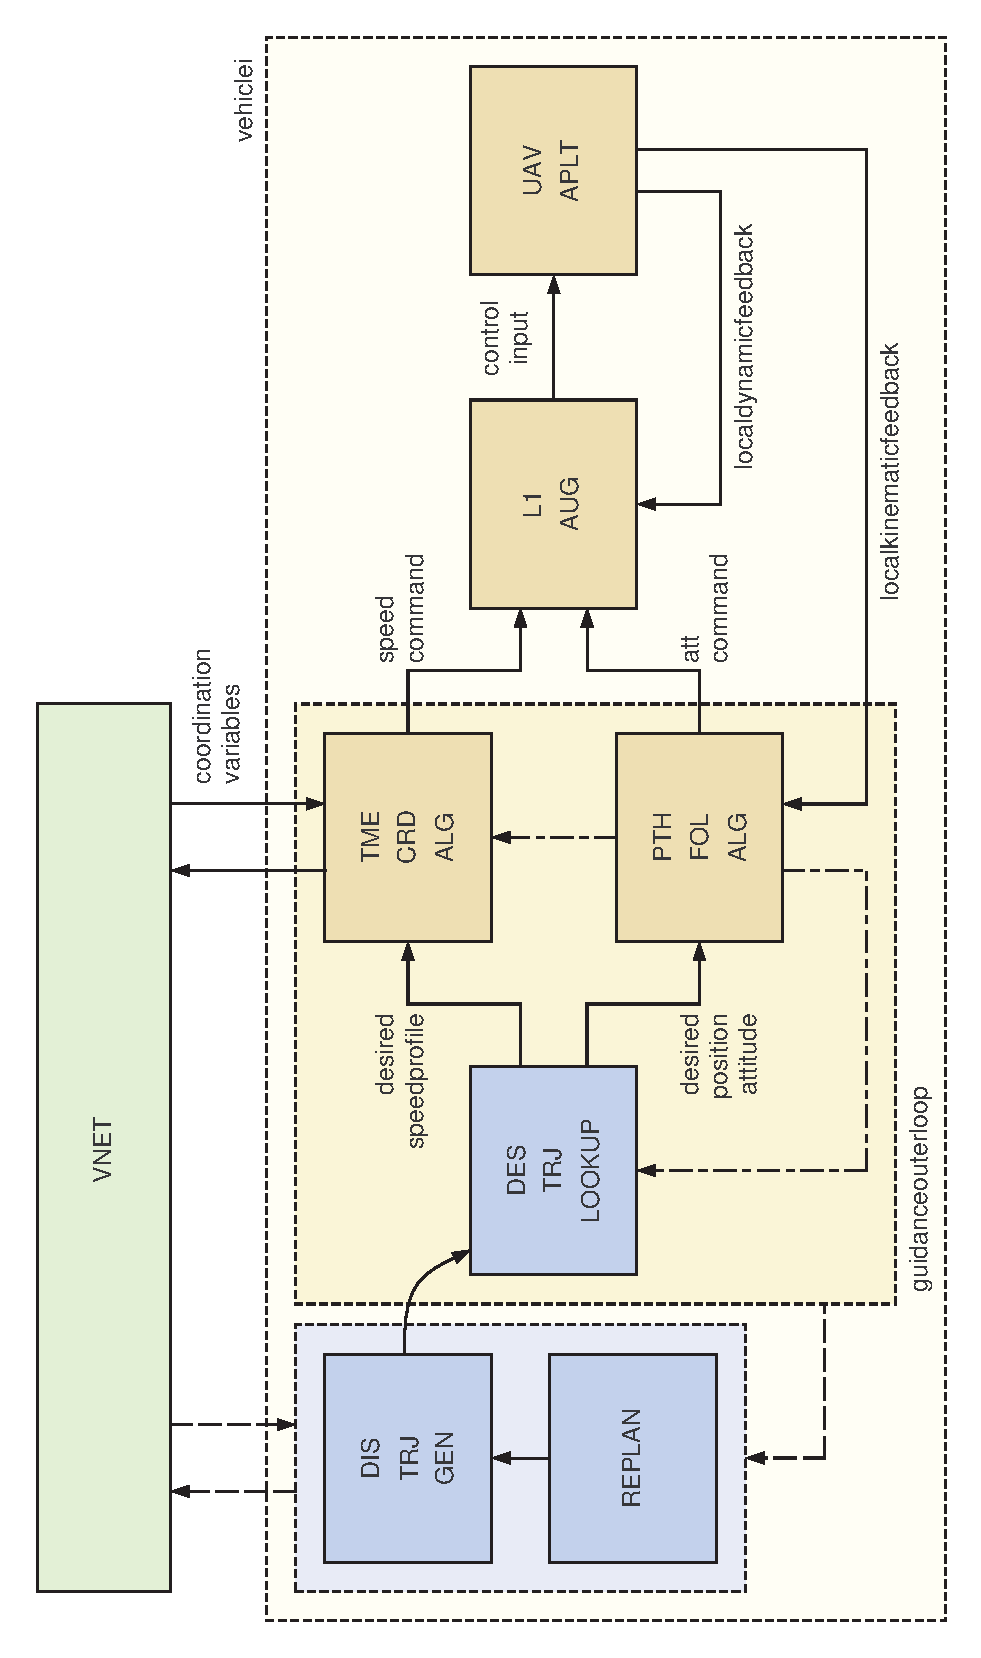
\includegraphics[width=0.57\textwidth,angle=-90]{figures/CPF/overallarchitecture.ps}
    %
    \vspace{2mm}
    \caption{Conceptual architecture of the cooperative control framework adopted.}
    \label{fig:overall_architecture}
    \vspace{3mm}
\end{figure}
%------------------------------------------------------------------------------


As part of the proposed solution, a \emph{path-following} nonlinear control algorithm has been proposed that uses vehicle angular rates to steer a vehicle along a desired 3D~spatial path for an arbitrary feasible temporal assignment along the path. The algorithm thus relies on the insight that an aircraft can follow a given path using only its attitude, thus leaving its linear speed as an extra degree of freedom to be used at the coordination level. The path-following control algorithm uses the special orthogonal group~$\mathsf{SO(3)}$ in the formulation of the attitude-control problem; this formulation avoids the geometric singularities and complexities that appear when dealing with local parameterizations of the vehicle's attitude and thus leads to a singularity-free path-following control law. Figure~\ref{fig:ScenPF_PFsequence} presents simulation results of a single vehicle mission scenario in which a small~UAV is tasked to follow a spatial path consisting of a left turn followed by a right turn, and climbing steadily from $200~{\rm m}$ to $400~{\rm m}$. Details about the path-following control law as well as additional simulation results can be found in~\cite{GNC11_PFSO3,XargayPhd}.


%--------------------------  FIGURE  ------------------------------------------
\begin{figure}[p]
    \centering
    \hspace*{-10mm}
    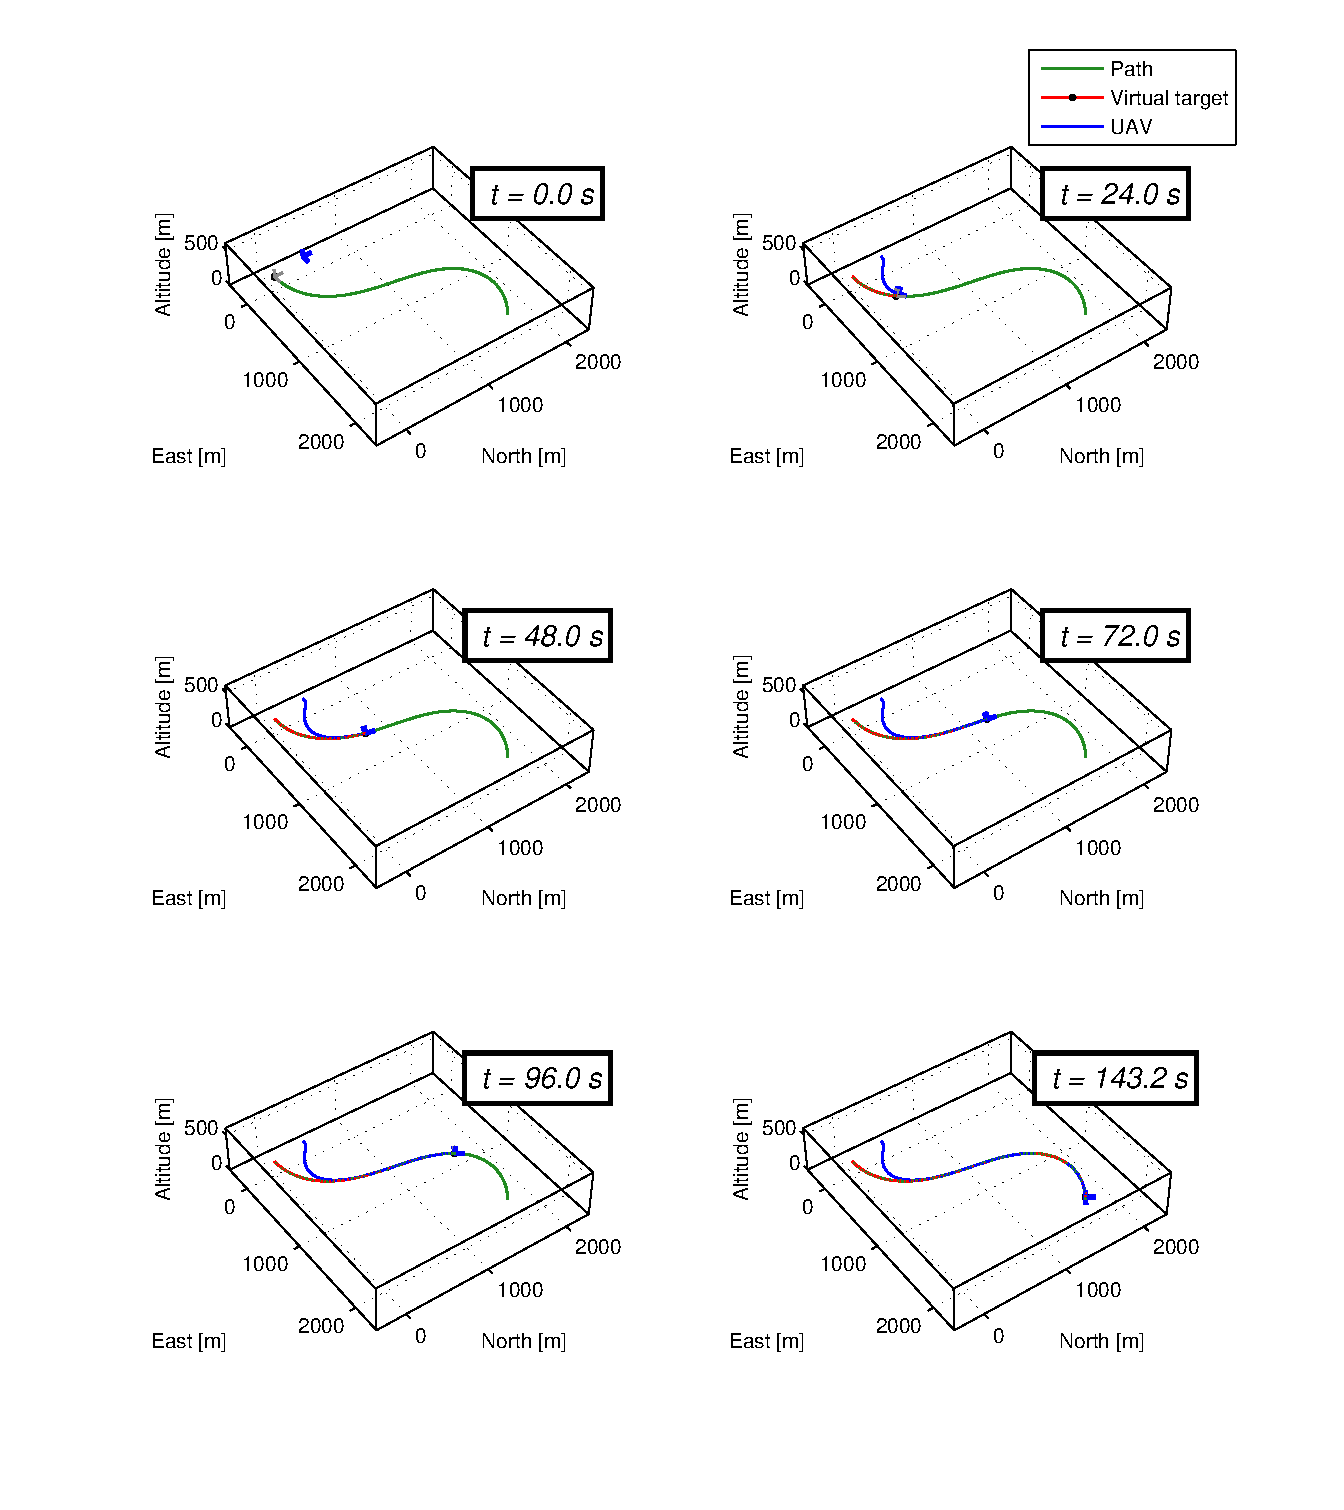
\includegraphics[width=\textwidth]{figures/CPF/Scen_pf3D.eps}\\[-5ex]
    \caption{Path following of a single UAV.}
    \label{fig:ScenPF_PFsequence}
\end{figure}
%------------------------------------------------------------------------------


To enforce the temporal constraints of the mission, a \emph{time-coordination algorithm} adjusts the speed profile of each aircraft based on coordination information exchanged among the vehicles over a supporting communications network. This coordination algorithm relies on a distributed control law with a proportional-integral structure, which ensures, first, that the fleet achieves the desired agreement and, second, that each vehicle travels along its path at the desired speed, and also provides disturbance rejection capabilities against steady winds. Moreover, this coordination control law can be implemented as a multi-leader protocol, which can improve the robustness of the cooperative control architecture to a single-point vehicle failure. Figure~\ref{fig:ScenCPF_CPFsequence} presents simulation results of a multi-vehicle cooperative mission scenario in which three small UAVs must execute sequential auto-landing while maintaining a pre-specified safe-guarding separation ($30~{\rm sec}$) as they fly along the glide slope. As can be seen in the figure, the path-following algorithm eliminates the initial offset in both position and attitude, and steers the UAVs along the corresponding paths, while the coordination algorithm ensures that the UAVs reach the glide slope separated by the desired time-interval. The UAVs reach the glide slope at ${t=67.2~{\rm sec}}$, ${t=97.1~{\rm sec}}$, and ${t=127.1~{\rm sec}}$, approximately meeting the desired $30~{\rm sec}$ inter-vehicle separation. After reaching the glide slope, the path-following algorithm ensures that the UAVs stay on the glide path as the coordination algorithm maintains the safe-guarding separation. Further details about the distributed coordination control law as well as additional simulation results can be found in~\cite{JGCD13_CPF,XargayPhd}.


%--------------------------  FIGURE  ------------------------------------------
\begin{figure}[p]
    \centering
    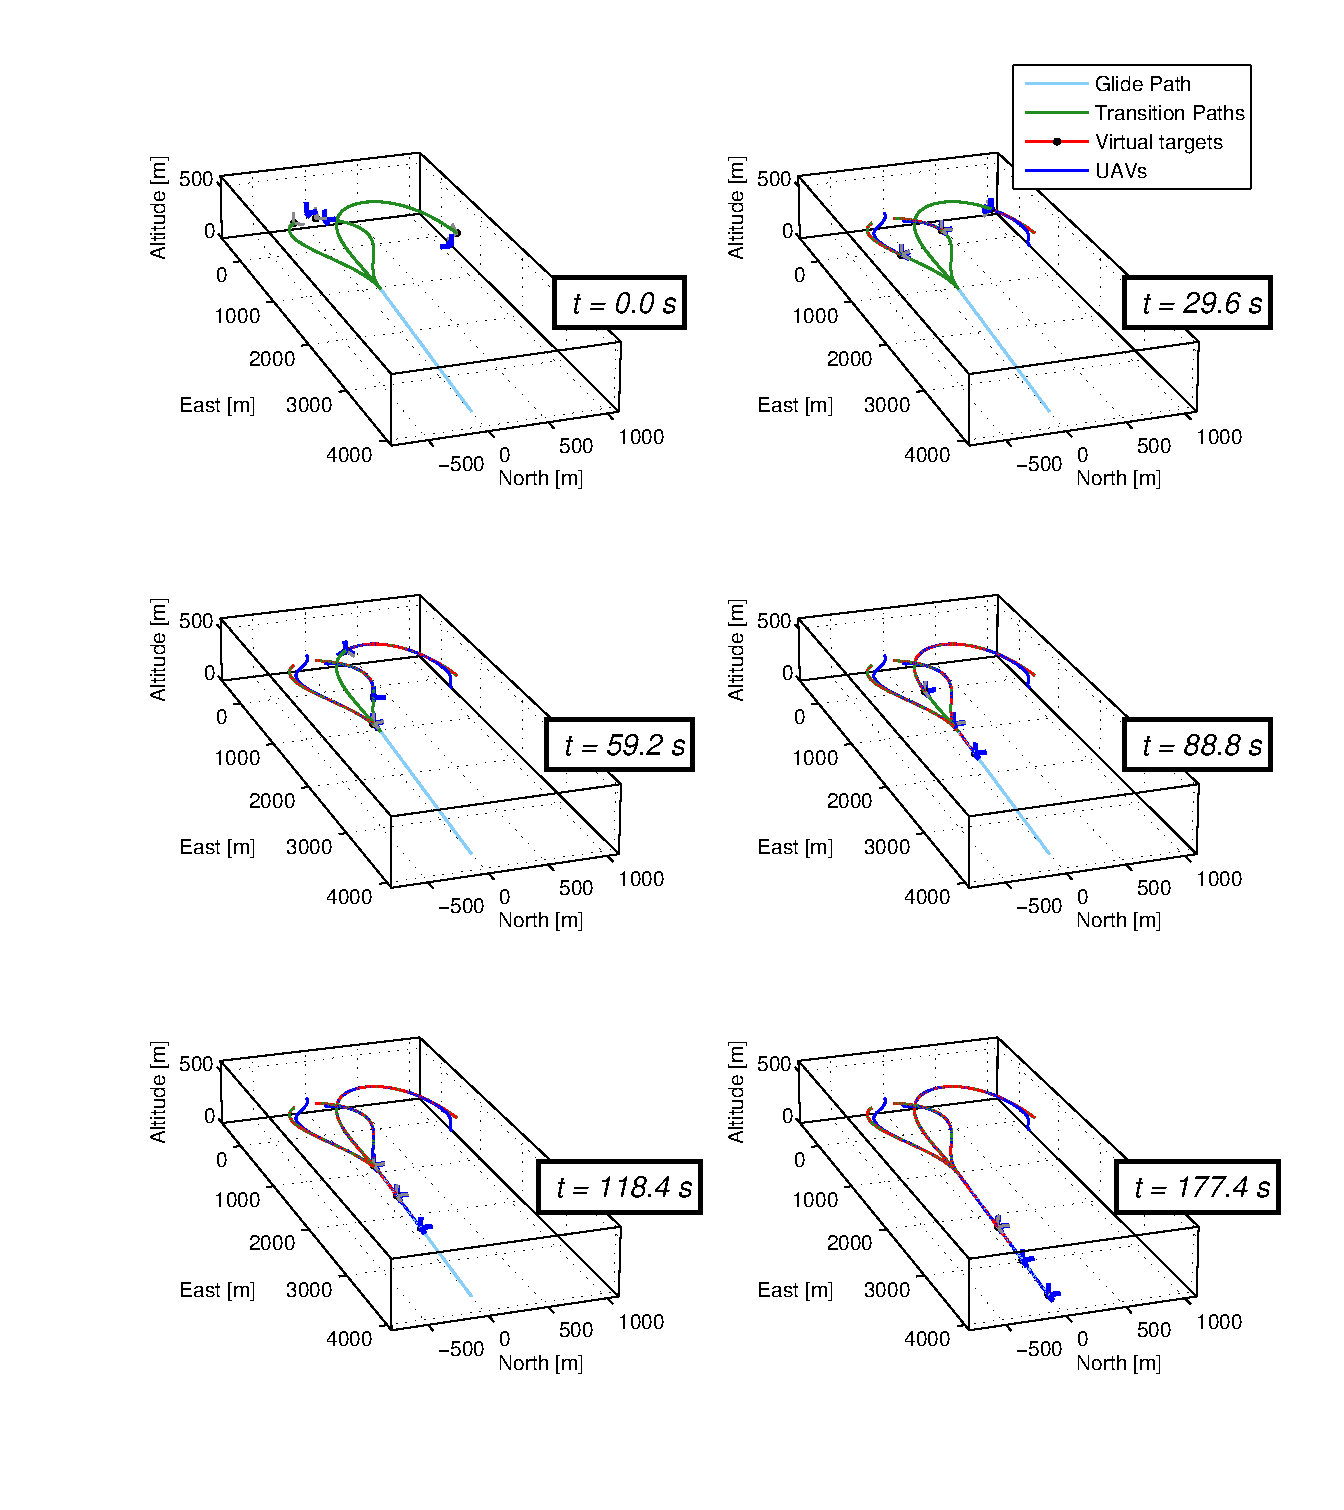
\includegraphics[width=\textwidth]{figures/CPF/Scen2_cpf3D.eps}\\[-5ex]
    \caption[Sequential auto-landing; mission evolution.]{Sequential auto-landing. The three UAVs arrive at the beginning of the glide path separated by approximately~$30~{\rm sec}$ and maintain this safe-guarding separation as they fly along the glide slope.}
    \label{fig:ScenCPF_CPFsequence}
\end{figure}
%------------------------------------------------------------------------------


These cooperative control algorithms have also been extensively flight tested at Camp Roberts, CA. In particular, a multi-UAV cooperative road-search mission was successfully completed during the quarterly run Tactical Network Topology\footnote{Information available online at \url{http://www.nps.edu/Academics/Schools/GSOIS/Departments/IS/Research/FX/CBETNT/CBE/TNT.html} [Online; accessed 8~March~2013]. See also~\cite{netzer09_TNT}.} field experiments conducted through the Field Experimentation Cooperative Program, which is being led by the U.S.~Special Operations Command and the Naval Postgraduate School. To visually illustrate the effect of time-critical cooperation among the UAVs, Figure~\ref{fig:FTs.coordframes} presents a mosaic of four consecutive high-resolution images taken during a flight-test experiment. In this experiment, the road-search paths are intentionally separated by altitude and optimized such that, if the coordination algorithm adequately adjusts the speed of the two UAVs, then the UAV flying at a lower altitude is expected to be continuously present in the field of view of the camera flying at a higher altitude. The figure schematically represents the progression of the lines of sight connecting the two cameras onboard the UAVs with a virtual target vehicle running along the road. Time-coordination ensures that cameras observe the same spot on the road and thus maximize the overlap of the footprints of their fields of view, which is critical to provide reliable target discrimination. Additional flight-test results have been presented and described in detail in~\cite{CSM12_CPF}.


%--------------------------  FIGURE  ------------------------------------------
\begin{figure}[h]
    \centering
    \includegraphics[width=0.9\textwidth]{figures/CPF/FTs_4pics.eps}
    %
    \vspace{3mm}
    \caption[Time-critical cooperation in a road-search mission.]{Time-critical cooperation in a road-search mission. In this experiment, the road-search paths are intentionally separated by altitude and optimized such that the UAV flying at a lower altitude is continuously present in the field of view of the camera flying at a higher altitude. A mosaic of four consecutive high-resolution images illustrates the progression of the lines of sight~(LoSs) connecting the two onboard cameras with the virtual target vehicle running along the sensor path.}
    \label{fig:FTs.coordframes}
\end{figure}
%------------------------------------------------------------------------------


%------------------------------------------------------------------------------
\subsubsection{Coordination Performance Guarantees under Adverse Communication Conditions}

Success of the time-critical, multi-vehicle, cooperative missions described above depends on the ability of the team to exchange information in a timely and reliable manner and, therefore, the \emph{quality of service}~(QoS) of the supporting communications network becomes a factor of major importance. Previous research efforts in this area by the Co-PIs have led to the derivation of performance guarantees for various distributed coordination protocols in the presence of faulty communications networks. According to the obtained results, the guaranteed levels of performance are limited by the~QoS of the supporting network; see~\cite{CSM12_CPF,CDC12_QuadCPF,JGCD13_CPF,XargayPhd}. The work in~\cite{XargayPhd}, for instance, derives lower bounds on the rate of convergence of the closed-loop coordination dynamics with the proportional-integral protocol mentioned in the previous section as a function of the level of connectivity of the communication network. In particular, this work assumes that the connectivity of the communications graph~$\Gcal(t)$ that captures the underlying bidirectional communications network topology of the fleet at time~$t$ satisfies the \emph{persistency of excitation} (PE)-like condition~\cite{PassivityCoord_Arcak}
\begin{equation}\label{eq:CommLim.PEcomm}
\frac{1}{n}\frac{1}{T} \int_t^{t+T} \bm{Q}\,\bm{L}(\tau)\,\bm{Q}^{\top}\,{\rm d}\tau \geq \mu \,\IIn{n-1}\,,
\qquad\qquad \mbox{for all}~t\geq0\,,
\end{equation}
where $n$ is the number of vehicles, ${\bm{L}(t)\in\IR^{n\times n}}$ is the Laplacian of the graph~$\Gcal(t)$, and $\bm{Q}$ is an ${(n-1)\times n}$ matrix such that ${\bm{Q}\bm{1_n}=\bm{0}}$ and ${\bm{Q}\bm{Q}^{\top}=\IIn{n-1}}$, with $\bm{1_n}$ being the vector in~$\IR^n$ whose components are all~$1$. Parameters~${T>0}$ and~${\mu\in[0,1]}$ characterize the~QoS of the communications network. We note that the PE-like condition~\eqref{eq:CommLim.PEcomm} requires the communications graph~$\Gcal(t)$ to be connected only in an integral sense, not necessarily pointwise in time\footnote{This connectivity condition is similar to the concept of \emph{uniformly joint connectivity} used in~\cite{lin07}.}. Under this connectivity assumption, it is shown in~\cite{XargayPhd} that the proportional-integral protocol guarantees the following rate of convergence of the closed-loop coordination error dynamics:
\begin{equation}\label{eq:CommLim.convrate}
\bar{\lambda}_{c} := \frac{k_{P}n\mu}{(1+k_{P}nT)^2}\,\left(1+\rho_{k}\frac{n}{n_{\ell}}\right)^{-1}, \qquad\qquad
\rho_{k}\geq2\,,
\end{equation}
where $k_{P}$ is the proportional coordination control gain, $n_{\ell}$ is the number of leaders included in the coordination control law, and $\rho_{k}$~is a design variable related to the integral coordination control gain~$k_{I}$. Clearly, the guaranteed rate of convergence of the coordination control loop is limited by the~QoS of the communications network. This implies that, in communication-limited environments, characterized by small parameters~$\mu$ and large parameters~$T$, long times might be required for the vehicles to reach the desired agreement. These unfavorable conditions can clearly lead to potential separation violations.

%\subsubsection{Online estimation of partially known coordination states resulted from low-communication conditions}
% this subsection proposes new development . It should go to

% -----------------------------------------------------------------------------
\subsection{The Framework for Prevention of Loss of Separation }
\label{subsec:framework}
% -----------------------------------------------------------------------------

\subsubsection{Overview of the Framework and the Task Statement}
The architecture of iSEALC framework proposed in this research effort adopts the concept and the key methods of coordinated path following that were introduced in the previous section. The iSEALC framework extends the developed  approach with algorithms and control schemes capable of rapidly identifying potential violations of separation assurance for given performance of heterogeneous aircrafts.

While the originally developed coordination algorithms provide robustness guarantees with respect to intermittent loss of communication the envisioned high density of future air-traffic and the complexity of networked communication still call for novel approaches that can accommodate unforseen conditions. To address this problem we propose to develop a set of onboard proactive estimators to improve the knowledge that each airplane (or node in the network of aircraft) has about the coordination states of other vehicles, while  broadcasting its own coordination state to its neighbors, as determined by the time-varying communications topology. The states of the local estimators can then be used by the decentralized control law to enforce vehicle coordination even during time-intervals when the actual coordination states of ''neighboring`` vehicles are not available. The use of local proactive estimators improves the convergence rate of the closed-loop coordination dynamics in low-connectivity scenarios.

The iSEALC framework addresses the following main airspace management problem:
%-----------------------------------------
\vspace{-2mm}
\begin{itemize}
\setlength{\itemsep}{-4pt}
    \item For a given geometrically bounded airspace sector that includes a given number of cooperative aircraft flying along the preassigned paths with nominal speed profiles, what are the pairs of paths that intersect in time?

    \item If a number of collisions in time is identified ahead of time and the aircraft exchange their coordination states over the faulty communication network characterized by the rate of loss of information [give a ref to PE condition], what are the control law and the minimal time to LOS event required to successfully adjust speed of aircraft involved to prevent the LOS event.
\end{itemize}
\vspace{-2mm}

A solution to these problems must necessarily involve the knowledge of the paths defined at the path planning step, where the an appropriate route optimization  problem is solved. Assuming that the knowledge of nominal paths and speed profile can be exchanged via broadcast of minimal number of path and speed defining parameters, results in a simple task of verifying if the paths intersect in time. Next, a complete solution must include a coordination algorithm between the aircraft that provides robustness to the execution of path following and separation assurance for the entire fleet in the presence of faulty communication networks.

In the following we present the building blocks of the proposed framework including the proactive estimators and the software infrastructure necessary to interface with the real ATC data.

%------------------------------------------------------------------------------
\subsubsection{Coordination Performance Improvement in Communication-Limited Environments}

Building on this past work of the Co-PIs, in this research effort we propose to develop novel distributed coordination control laws that improve the convergence rate of the coordination dynamics in communication-limited scenarios. Preliminary results in this direction are presented in~\cite{XargayPhd}, where a new protocol for improved vehicle coordination is proposed that brings together tools and concepts from control of complex networks, topology control, and logic-based communication protocols. In fact, the problem of designing a control law that speeds up the convergence of the coordination dynamics under low connectivity can be seen as the dual problem of determining a logic-based communication protocol that is able to reduce the amount of information exchanged over the network while maintaining a desired level of performance. Logic-based protocols use banks of local estimators and communication logics to determine when each node should communicate its own state to the neighboring nodes, and have been shown to significantly reduce the required channel bandwidth~\cite{TCST02_Tilbury,ACC04_Hespanha}. In~\cite{XargayPhd}, instead, the use of local estimators is intended to improve the \emph{knowledge} that each node has about the coordination states of other nodes, while continuously broadcasting its own coordination state to its neighbors, as determined by the time-varying communication topology. The states of the local estimators can then be used by the coordination control law to enforce coordination even during time-intervals when the actual coordination states of other nodes are not available.


Clearly, in this approach, the estimators are useful only if nodes receive ``enough'' information from the corresponding neighboring nodes; if this is not the case, then each vehicle is just carrying a bag of estimators with worthless information, which may reduce the convergence rate of the coordination error dynamics due to a ``large network effect''. This implies that precise a~priori knowledge about the (local) structure of the network topology would be beneficial for an effective implementation of such estimators. The framework envisioned in this research effort, however, assumes no information about the structure of the network topology, other than the ---rather general--- integral connectivity condition~\eqref{eq:CommLim.PEcomm}. This means that the vehicles in the fleet do not know in advance which neighbors they are going to exchange information with or the amount of information received from each neighbor. The question is thus how to design a coordination control law that can take advantage of the additional information provided by the estimators without experiencing the drawbacks associated with a large extended network.


To address this problem, preliminary work in~\cite{XargayPhd} develops strategies to control communication links between each node and its estimators. These topology-control strategies are thus responsible for deciding when an agent should ``listen'' to a particular estimator and adjusting the corresponding link weight accordingly. Various approaches can be investigated for topology control, ranging from a \emph{hybrid strategy} in which links switch between different activation/deactivation modes to a continuous strategy based on \emph{edge snapping}~\cite{TCS10_DeLellis,CHAOS11_DeLellis}. In any case, this cooperative framework leads to an evolving network, whose (directed) topology depends on the local exchange of information among nodes. The results reported in~\cite{XargayPhd} provide numerical evidence suggesting that, with this new approach, the coordination error state converges to a neighborhood of the origin in a shorter time. Figure~\ref{fig:tccLC.MCruns.hist} presents the histograms and distribution fits of the normalized convergence time of the coordination error dynamics for 1,024~Monte~Carlo runs of the sequential auto-landing mission scenario described earlier in this proposal using both the hybrid approach and the edge-snapping strategy. In addition, the figure also shows \emph{generalized extreme value}~(GEV) distribution fits to these histograms~\cite{GEVbook}. The location, scale, and shape parameters (conventionally denoted in the literature as~$\mu$, $\sigma$, and $\xi$) characterizing these two GEV~distribution fits are summarized in Table~\ref{tbl:tccLC.MCruns.GEVfit}. The table also contains estimates of the mean of both distributions, which indicate that, in average, the hybrid approach is able to reduce the convergence time to a~$43\%$ of the original value, while the edge-snapping strategy shortens the convergence time to a~$51\%$ of this value.


%--------------------------  FIGURE  ------------------------------------------
\begin{figure}[h]
        \centering
        \begin{subfigure}[b]{0.45\textwidth}
                \centering
                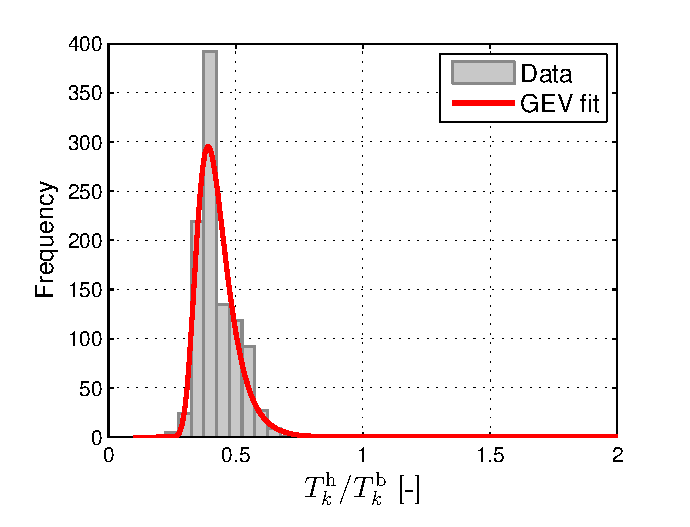
\includegraphics[width=\textwidth]{figures/CPF/Scen2_cpfMC_histHY.eps}
                \caption{Hybrid approach}
        \end{subfigure}%
        \hspace{5mm}
        \begin{subfigure}[b]{0.45\textwidth}
                \centering
                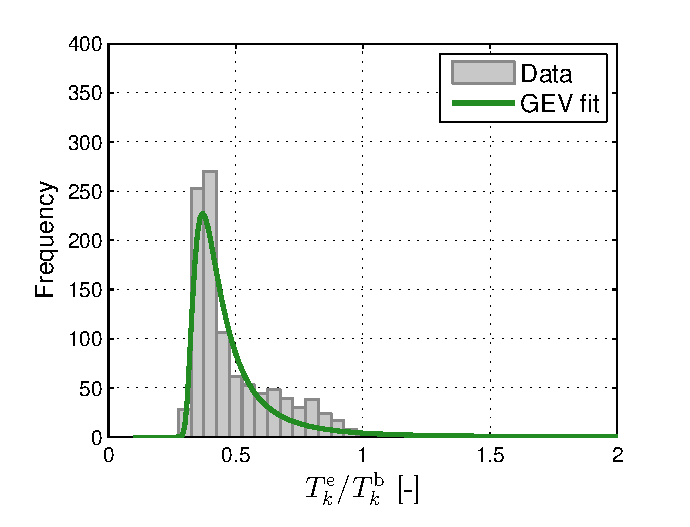
\includegraphics[width=\textwidth]{figures/CPF/Scen2_cpfMC_histES.eps}
                \caption{Edge Snapping}
        \end{subfigure}%
        %
        \vspace{2mm}
        \caption[Histograms and distribution fits of the normalized convergence time.]{Histograms and distribution fits of the normalized convergence time of the coordination error dynamics with both the hybrid approach and the edge-snapping strategy.}
        \label{fig:tccLC.MCruns.hist}
        \vspace{6mm}
\end{figure}
%------------------------------------------------------------------------------

%--------------------------  TABLE  -------------------------------------------
\begin{table}[t]
    \centering
    %
    \caption[Characterization of the GEV~distributions in Fig.~\ref{fig:tccLC.MCruns.hist}.]{Mean, variance, as well as location, scale, and shape parameters characterizing the two GEV~distributions in Figure~\ref{fig:tccLC.MCruns.hist}.}
    \label{tbl:tccLC.MCruns.GEVfit}
    %
    \renewcommand{\arraystretch}{1.2}
    %
    \begin{tabular}{c | c c | c c}
    \hline\hline
    \hspace{1cm} & \multicolumn{2}{c|}{Hybrid} & \multicolumn{2}{c}{Edge Snapping} \\
    & \emph{Estimate} & $95\%$ \emph{confidence} & \emph{Estimate} & $95\%$ \emph{confidence} \\
    \hline
    $\mu$ & $0.3925$ & $(0.3887,0.3964)$ & $0.3967$ & $( 0.3914,0.4020)$ \\
    $\sigma$  & $0.0583$ & $(0.0556,0.0611)$ & $0.0763$ & $(0.0714,0.0815)$ \\
    $\xi$  & $0.0152$ & $(-0.0139,0.0442)$ & $0.4656$ & $(0.4072,0.5239)$ \\
    \hline
    Mean     & 0.4270 & -- & 0.5051 & -- \\
    Variance & 0.0058 & -- & 0.3021 & -- \\
    \hline\hline
  	\end{tabular}
\end{table}
%------------------------------------------------------------------------------


\subsubsection{Functionality of the Framework and its Key Elements}
\label{subsubsec:functionality}
It is assumed in the following that the aircraft exhibit nominal flight performance and can accelerate and decelerate, climb and descent with nominal known characteristics.  Although degradation of flight dynamics characteristics is out of scope of this proposal, the originally developed CPF framework also addresses this problem and therefore corresponding tolls and methods can easily extend the solution proposed by iSEALC framework.

The envisioned functionality of iSEALC framework is based on the following key elements (see Figure\ref{fig:KeyAlg} for illustration):
%
%--------------------------  FIGURE  ------------------------------------------
\begin{figure}[thpb]
\centering
\vspace{-0mm}
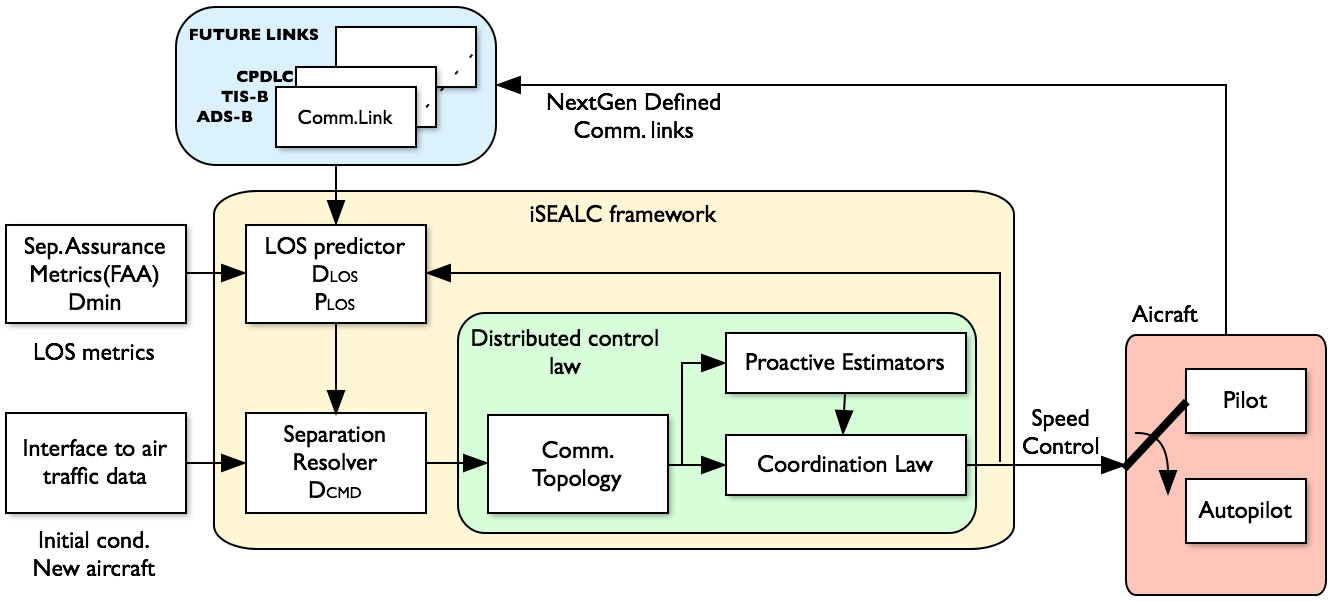
\includegraphics[angle=0,width=0.8\textwidth,]{key_alg.eps}
\caption{Key functional elements of the iSEALC framework.}
\label{fig:KeyAlg}
\end{figure}
%------------------------------------------------------------------------------
\vspace{-1mm}

%------------------------------------------------------------------------------
%------------------------------------------------------------------------------
\begin{itemize}
\setlength{\itemsep}{-1pt}
\vspace{-2mm}

\item \textbf{\emph{Distributed coordinated control law (DCL)}:} The DCL is the baseline coordination controller that takes as an input the actual communication topology of ''neighboring`` aircraft, their relative position (coordination variable) on the path, the desired separation matrix $D_{cmd}$ (will be defined by the separation resolver),  and produces the speed adjustment advisories for the pilot or the reference command for the onboard autopilot. The objective of the controller is to achieve consensus of coordination variables transmitted over faulty network, thus to force multiple aircraft to fly along their path in coordination. The set point of this control law (''virtual leader``) is defined based on the desired ''throughput`` that can be set either for the entire route or for the sequence of sectors that contain the route.  The ''neighboring`` aircraft is the one that has an intersecting route within the flight time of analyzed vehicle.

The controller assumes that the own aircraft flight dynamics characteristics are given (for example $min$ and $max$ speed), the performance characteristics of ''neighboring`` aircraft are known as they are communicated over the underlying network. As it is presented in~\cite{CSM12_CPF} the control law guarantees convergence of coordination variables and robustness of the controller to the loss of communication over a bounded period of time; in other words the rate of convergence of the coordination control loop is limited by the QoS of the communications network.

\item \textbf{\emph{Proactive state estimator of neighboring aircraft (PNE)}:} The PNE is an onboard estimator that is developed to improve the knowledge that each airplane (or node in the network of aircraft) has about the coordination states of other vehicles, while  broadcasting its own coordination state to its neighbors, as determined by the time-varying communications topology. The states of the local estimators can then be used by the DCL law to enforce vehicle coordination even during time-intervals when the actual coordination states of ''neighboring`` vehicles are not available. The use of local PNE estimators improves the convergence rate of the closed-loop coordination dynamics in low-connectivity scenarios. The input to the PNE is the same as the input to the DCL law - the communication topology and the coordination variables.

Besides improving  the convergence rate of the coordination dynamics, the PNE estimators introduce novel strategies that control the communication links between each vehicle and its estimators; in other words, PNE defines the desired rate of communication and defines the conditions of when to transmit and when to listen the coordination states. This approach leads to an evolving network, whose topology depends on the local exchange of information among the ''neighboring`` nodes.

\item \textbf{\emph{Predictor of LOS event (LOS)}:} The LOS predictor is an open-loop ''integrator`` that dead reckons the speed dynamics of all airplanes that communicate their state(position on the path), current speed and the intent (parameterized path). The time of integration is defined by the ''neighboring`` aircraft that is positioned at the longest distance from the own craft. The LOS predictor runs online and at every instance of time produces two matrices: first is the matrix of minimal predicted distances $D_{min}$ among the surveyed aircraft, and second is the matrix of corresponding relative positions on the path $P_{LOS}$. Based on the comparison of $D_{min}$ with FAA defined minimal separation bounds $D_{req}$ for different types of scenarios( aircraft and airspace type) the LOS predictor calculates a binary matrix of potential separation violations $B_{LOS}$ that along with $P_{LOS}$ uniquely identifies the aircraft involved, routes, and the relative time to collision.

Similarly, a second LOS predictors can be run in parallel to verify for example the ''worst case scenario`` of interest. In particular, assuming that all ''neighboring`` aircraft initially know their  position on the path but there might be a deviation of speed of given magnitude and loss of communication of chosen duration, the LOS algorithm can produce the result that predicts a possibility of separation violation at much earlier time.

\item \textbf{\emph{Separation Resolver (SR)}:} Before submitting the matrix of potential LOS events $B_{LOS}$ to the DCL law for automatic speed adjustment, the system needs to address the task of ordering the aircraft on their paths and injecting a new aircraft into the queue; the aircraft that completes its flight, automatically does not have any neighbors and thus leaves the queue and the coordination network.

The SR performs ordering of the aircraft along the normalized path by adding the required separation distance (normalized) to the coordination variable (relative position on the path) of conflicting airplane. Resulting matrix $D_{cmd}$ obtained across all ''neighboring`` aircraft is the reference command to be followed by the CDL law.

Injecting a new aircraft into the queue is performed by finding the closest (in time) place in the existing queue that does not have any conflicts with the neighbors. Solving this task requires the knowledge of aircraft flight performance characteristics such as $max$ and $min$ values of climb and descent rates, and acceleration deceleration characteristics.

\end{itemize}

In the  following subsection we discuss the overall functionality of the proposed framework and possible solutions for the design and implementation of this technology.

\subsubsection{Operational Modes}

We envision that the proposed system can be used in two operational modes. First it can be utilized as a ground based separation assurance tool. In this mode the primary objective is to serve as an ATC advisory tool to help identifying potential LOS events ahead of time so that there will be no need to change the paths of conflicting airplanes. More precisely, if the routes and nominally assigned speed profiles of all airplanes are known, then cooperative execution of the nominal routes and coordination of states along the paths with possible adjustment of speed should be sufficient to prevent LOS events.

Second, the proposed framework can be also implemented onboard of aircraft either as a separation advisory tool or as a standalone speed coordinating controller. The key algorithms would be the same, however depending on the equipage of a specific aircraft some computationally heavy algorithms might be omitted.

The system initialization in both modes should be the same. The framework can be initialized with a ''snapshot`` of current state of an airspace sector containing the number and type of aircrafts, their declared routes and nominal temporal assignments (speed profiles). The FAA dictated minimum separation assignments $D_{req}$ for different type of aircraft and airspace types are assumed be known. Thus when the system is initialized or a new aircraft enters the considered segment the separation matrix is either built to match the number of aircraft or extended by one with the  separation values assigned to the corresponding pairs of aircrafts in the segment. As soon as the system is initialized the algorithms perform re-parameterization of the states, routes, and the speed control assignments in terms of primitives utilized by the CPF framework. Right at this stage the dimension of the separation assurance space significantly reduces thus making the solution of separation assurance task feasible to obtain in close to real-time pace.


\subsubsection{Ground-Based Assessment Mode}

When utilized in \textbf{\emph{''the worst case scenario``}} mode the system runs along the  parameterized paths with the predefined dynamics of aircrafts and evaluates the matrix of separation distances $D_{min}$ for all pairs of aircraft in the chosen airspace segment  and in the presence of simulated adverse communication conditions caused by the capabilities of individual and integrated data broadcast systems.

Assuming that airborne aircraft might execute the same feedback control algorithms that are implemented on the ground, it is sufficient to identify the maximum severity of the loss of communication before there is no speed control action that can resolve the separation conflict. Thus starting with an initial combination of communication failures and speed deviations the framework obtains the binary matrix of potential separation violations $B_{LOS}$ and associated $P_{LOS}$ along with the coordination law that strives to avoid the loss of separation. If  the speed control for each aircraft is capable of preventing the loss of separation then the simulated adverse communication conditions can be ''worsened``. Thus following the ideas of $\gamma$-Iteration method from Robust Control ~\cite{zhou1998essentials} the procedure can be iterated until the capabilities of speed control of the aircraft in LOS condition are not sufficient to guarantee desired separation.

Interpreting the resulting speed coordination law (computed by the DCL module on the ground) resulting from the worst case scenario would be analogous to the control law in the robust control task that maximizes the magnitude of disturbance caused by the low connectivity condition across all available communication channels with the assumption that speed of each aircraft can be varied in a given interval.
%As introduced before, the resulting separation matrix $D_{min}$ that represents the minimal separation distances between
%the $i$ and $j$ airplane pairs can be naturally used as the metric for separation assurance. The minimum value of entries
%of this metric are compared to the minimal distances nominally required by the FAA for each type of aircraft identified in
%possible violation of separation bounds.

Obviously, that ``the worst case scenario'' might result in a number of ''panic`` pairs of the separation matrix $B_{LOS}$. All of the ''panic pairs`` are the advisories for the ATC system and need to be monitored.

To automate the monitoring process the same algorithms of iSEALC framework need to be utilized in \textbf{\emph{''monitoring``}} mode when the system as before runs online and is updated by real data coming from all aircrafts in the considered segment. The varying communication conditions resulted from low connectivity or even loss of communication will necessarily result in adjusting the nominal speed control laws assigned to the aircrafts at the initialization stage. However, the DCL architecture and the distributed nature of the speed coordination law will timely adjust the speed profiles of each aircraft in a potential separation violation condition identified by the ''worst case scenario``. As long as the coordinated control law is not saturated (saturation bounds are different for each type of aircraft)  for the entire flight time the ''panicked`` mode will not be confirmed. In turn, if the control law of a specific aircraft is saturated all the time, then the panicked mode is confirmed and the corresponding advisory is given ahead of time to the ATC personnel with detailed specification of time to possible violation of separation bounds. This alarming condition still does not confirm the fact of collision as the onboard TACAS or ADS-B and other systems still provide pilots and onboard intelligence with sufficient information to avoid a collision. In this sense the proposed system is complementary to the available capabilities.

\subsubsection{Onboard Implementation}

To achieve the most effective mode of operation the iSEALC system can be integrated onboard aircrafts as an automated monitoring, advisory and control system. In this \textbf{\emph{''onboard mode``}} the system relies on cooperative sharing of state and intent information across the network of entire fleet of aircrafts in a chosen airspace segment. When implemented onboard the system automatically adjusts the speed profiles of each and all aircrafts in the segment and guarantees that every vehicle follows its predefine path with the speed that guarantees the desired separation matrix. To achieve significantly higher level of situational awareness and LOS resolution we propose to develop and implement onboard an additional level of online PNE estimators of the states of all neighboring aircrafts. As described above, this proactive estimators run in parallel with the coordination law and estimate the states of the neighboring aircrafts while accounting for the degraded communication. The original coordination control law is thus extended with the estimated states of aircrafts nearby and thus provides higher robustness to low connectivity conditions.

% -----------------------------------------------------------------------------
\subsection{Verification and Validation}
% -----------------------------------------------------------------------------

In order to validate the effectiveness and performance of the proposed research in preventing separation violation, the iSEALC system will be first validated in the Software-in-the-Loop~(SIL) and Hardware-In-The-Loop (HIL) flight simulations using computational and hardware capabilities~\cite{dobrokhodov2013RFCPS} of the NPS and UIUC team. The focus of this phase will be in the preliminary evaluation of the developed control strategies, their performance and the computational feasibility. The team also proposes to employ the advanced capabilities of the Air Traffic Control  and Future Flight Central(FFC) Simulators available at NASA Ames research center\cite{prevot2003distributed}, which provide high realism ATC environment from the perspectives of both the ATC controllers and the aircraft crew. The objective of this step is to prove the concept of distributed coordinated  control in a manned aircraft domain.

\subsubsection{SIL and HIL Experiments}
NPS and UIUC teams have significant computational and rapid control prototyping tools and facilities to enable initial validation and verification of the developed distributed control strategies. The key technological objective of verification is to evaluate the theoretically predicted performance of the distributed control law.

The UIUC/NPS team has been actively collaborating for the past decade and acquired significant knowledge in the theoretical aspects and in flight validation and verification of advance control strategies primarily focusing on unmanned platforms. Although being successful in flight management of multiple research unmanned aircraft capable of long duration flight, and closely interacting with the professional ATC community, we realize that our experience in the manned aircraft domain is limited. Therefore we propose to start interaction with the targeted community of ATC controllers at NASA Ames center at the early stage of project development. The objectives are twofold. First, this interaction enables solid understanding of the practical issues associated with current communication technologies (their mode of operation, technological and performance limitations) onboard and on the ground. Second, this interaction will help formulating the most representative case studies that should be implemented in the SIL and HIL simulations.

Utilizing the case studies developed at this stage we plan to integrate the distributed control laws onboard the flight control system of research UAVs, while simultaneously executing the iSEALC framework as a ground-based separation assessment tool. Experimental evaluation of the system in real-time computational environment should be instrumental in evaluating the performance of coordination algorithms as a tool for LOS assessment.


\subsubsection{Technology Transition to NASA}

We propose to transition the developed framework to the advanced facilities of NASA Ames research center, and in particular to the NASA SimLabs ATC and FFC simulators\cite{prevot2003distributed}. Both simulators provide the highest possible fidelity of simulating the various aspects of air traffic management from the ATC controller's and crew's perspectives. Developing software interfaces to ATC/FFC simulators to enable verifying the capabilities of iSEALC framework would greatly benefit the outcomes of the project. The fundamental objective of this evaluation is in providing a proof of concept through qualitative and quantitative measurements of separation bounds, workload, efficiency of the coordination control law for various types of aircraft under realistic conditions.

% ===== end Technical Approach and Methodology   ==============================



% =============================================================================
\section{Impact and Relevance of the Proposed Research}
% =============================================================================
A fundamental design requirement for the NextGen air traffic control system is a highly reliable and safe method for automating separation assurance. The iSEALC concept departs significantly from the current methods of separation assurance, which primarily focus on mid to short term identification and detection of loss of separation with simplistic mitigation strategies. In contrast the iSEALC architecture offers fundamentally new approach to separation assurance that is based on the 4D trajectory management, collaborative route planning, new separation modes that are based on distributed speed coordination, the system-wide network-based information management while preserving key safety requirements of the system in the degraded communication conditions. The objective of the proposed solution is to enable coordination of multiple aircraft through integration of a unified distributed coordinated control law that is constantly active throughout the entire flight. The iSEALC distributed framework of identical cooperative controllers is persistently predicting the LOS event for each and all aircraft in the fleet. Hence, rather than intervening sequentially at the last moment and possibly leading to the loss of separation and even mid air collision, the system reacts as a normal feedback control law providing its desired performance and robust guarantees. We hope that, given both the opportunity to contribute to the program and appropriate level of funding, the solutions proposed by us can be matured and transitioned from the flight of multiple R\&D UAVs to the real operational environment of NASA Ames research center.

% ===== end Impact and Relevance   ============================================

% =============================================================================
\section{General Plan of Work}
% =============================================================================

% -----------------------------------------------------------------------------
\subsection{Key Milestones}
% -----------------------------------------------------------------------------

Within the next thirty-six months, if funded, the team of co-Is of this proposal will be working on the development of iSEALC framework. We hope that starting in the second year we will conduct an extensive evaluation of iSEALC in the SIL and HIL simulation environments at UIUC and NPS. We propose the following scheduler with the understanding that the time frames for these milestones can be refined based on our interaction NASA personnel.

\textbf{Year I:} We will work on synthesizing the iSEALC architecture including its onboard and the ground segments.
Furthermore, we will choose and analyze in detail the individual and integrated failure space of 1-2 onboard communication
technologies defined by the NextGen.
%------------------Year I-----------------------
\vspace{-3mm}
\begin{itemize}
\setlength{\itemsep}{-4pt}
    \item Xargay will work on the development of proactive estimators that will significantly improve the knowledge that each airplane (or node in the network of aircraft) has about the coordination states of other vehicles.

    \item Hovakimyan will collaborate with Xargay on the development of theoretical proofs of performance of proactive estimators and the integration of the corresponding solutions into the iSEALC software environment.

    \item Dobrokhodov will work on the design of the predictor of the LOS events and the separation resolver. Solution of both tasks will require knowledge of current ATC operational procedures for en route and terminal airspace support, FAA regulations regarding the classes of airspace, types  of aircraft, and their communication instrumentation. This work should result in a software solution that implements both models.

    \item Kaminer will collaborate with Dobrokhodov on the development of analytical models that implement the LOS predicting solutions.

    \item Jones will analyze the set of existing communication technologies defined by NextGen. He will design a case study for 1-2 data broadcasting units with the objective of identifying its operational modes and associated performance limitations. The nomenclature of the communication technologies of primary interest will be identified via collaboration with NASA colleagues. He will also collaborate with Dobrokhodov in the overall design of iSEALC software architecture.
\end{itemize}
\vspace{-2mm}

\textbf{Year II:} We will concentrate on developing the key building blocks of the iSEALC software architecture
including its onboard and the ground segments. The ultimate goal of this year is to integrate the key functional
components as discussed in ~\ref{subsubsec:functionality} into one software environment. Efforts for this year
should also result in a set of representative airspace configuration scenarios that will be used during the last
year of experimental validation studies.
%-------------------Year II----------------------
\vspace{-3mm}
\begin{itemize}
\setlength{\itemsep}{-4pt}
    \item Xargay and Hovakimyan will work on the analysis of theoretical performance guarantees of the extended distributed coordination law that integrates the nominal baseline speed coordination and the newly developed proactive estimators. Xargay will also contribute to the software integration of the extended control law.

    \item Dobrokhodov will work on the software integration of the developed LOS predictor, separation resolver and the extended control law into one unified software solution.

    \item Dobrokhodov will collaborate with Jones and Xargay to implement onboard the extended decentralized control law using the capabilities of the Rapid Flight Control Prototyping environment with its flight testing at restricted airspace in Camp Roberts, CA. two most representative airspace management scenarios will be implemented by 2 research UAVs.

    \item Kaminer will collaborate with Jones on the formal description of the individual and integrated failure space of the onboard communication solutions explored in the first year os studies. The objective of the effort is to produce a representative set of the ''worst case`` scenarios that will be utilized by the iSEALC run as a ground-based separation assessment tool.
\end{itemize}
\vspace{-2mm}

\textbf{Year III:} We will focus on final software integration of the iSEALC framework with software interfaces that
enable SIL and HIL experimental verification studies. This verification should be performed against the airspace
configuration scenarios defined in the previous year. Special attention will be given to developing interfaces with
NASA Ames high fidelity simulation environments. The ultimate goal of this year is to perform intensive validation
of the iSEALC framework in the most challenging airspace management scenarios presented by the ATC and FFC simulators
at NASA Ames.
%-------------------Year III----------------------
\vspace{-3mm}
\begin{itemize}
\setlength{\itemsep}{-4pt}
    \item Dobrokhodov will develop software interfaces to enable SIL and HIL experimental verification of the iSEALC framework. Together with Xargay and Jones they will perform initial experimental evaluation of the framework against the ''worst case`` studies of onboard communication equipment and the most representative scenarios of air space configuration. Further , they will perform the experimental studies at NASA Ames facilities following the experimental evaluation plan developed in SIL/HIL studies.

    \item Dobrokhodov will collaborate with Jones and Xargay to implement onboard the extended decentralized control law using the capabilities of the Rapid Flight Control Prototyping environment with its flight testing at restricted airspace in Camp Roberts, CA. two most representative airspace management scenarios will be implemented by 2 research UAVs.

    \item Hovakimyan and Kaminer will work closely with NASA specialists to design the case studies and scenarios to be later tested on NASA Ames facilities.

    \item All four members of the team will cooperate on the refinement of iSEALC based on the evaluation feedback obtained at NASA, and will finalize first release of iSEALC to NASA.
\end{itemize}
\vspace{-2mm}

\textbf{Reporting:} It is anticipated that reporting of the results will be done to NASA on as-needed basis. Moreover, a yearly progress report will be filed, as well as an end-of-project report detailing all the findings. Results will also be published in conferences and archival journals.

% -----------------------------------------------------------------------------
\subsection{Management Structure}
% -----------------------------------------------------------------------------

Naira Hovakimyan will be the PI on this proposal. She will closely collaborate with Enric Xargay, Isaac Kaminer, Vladimir Dobrokhodov, and Kevin Jones. Enric Xargay will assist in developing the proactive estimators and their analytical integration with the baseline coordination control law. Vladimir Dobrokhodov will assist in software integration of the theoretical findings. Isaac Kaminer and Kevin Jones will assist in analysis and evaluation of communication technologies and their limitations. This should result in identification of the individual and cumulative failure spaces of communication technologies defined by the NextGen. Their findings will help designing the ''worst case`` scenarios for the evaluation of iSEALC performance as a ground-based separation assessment tool. Naira Hovakimyan will be working with Enric Xargay of analytical proofs of  performance of the newly developed extended coordination control law. Budget is allocated to support two trips per year by the PI and one of the co-Is to NASA meetings and facilities.

% -----------------------------------------------------------------------------
\subsection{Data-Sharing Plan}
% -----------------------------------------------------------------------------

All developed materials, including relevant literature reviews, algorithms, proofs, software, and design of specific experiments, will be shared with NASA by the co-Is of this proposal through regular bimonthly reports. All deliverables under the contract will be provided to NASA with unrestricted/unlimited rights. The co-Is will closely collaborate with NASA engineers, since the proposed work includes validation of the developed technologies on NASA research facilities. Therefore, the co-Is will ensure that all materials will be shared and adhere to NASA guidelines. Additionally, all computer code modules will be compatible with NASA software for further integration. In doing so, the co-Is strive to enhance the knowledge transfer and long-term value of the proposed work to NASA. Results will be submitted for publication to the AIAA~Guidance, Navigation, and Control Conference.

% ===== end General Plan of Work   ============================================


% ==============================================================================
% =====   PROPOSAL ENDS HERE   =================================================
% ==============================================================================



\clearpage
\pagenumbering{arabic}
% ==============================================================================
\bibliographystyle{ieeetran}
\bibliography{nasa_nra}
% ==============================================================================

\end{document} 